\chapter{Introduction}

\section{Overview}

Rephotography or repeat photography denotes the retrieval of the precise viewpoint used for taking a
--- possibly historic --- photograph and capturing another image from the same
spot, ideally with the same camera parameters. This allows for documentation and
visualisation of changes which the scene has undergone between the two or more
captures.  For instance when documenting urban development, one can present
progress of construction, restoration efforts or changes in the surroundings in
a visually striking manner, e.g. by blending the photographs together.
Figures \autoref{fig1} and \autoref{fig2} show examples.

\begin{figure}
   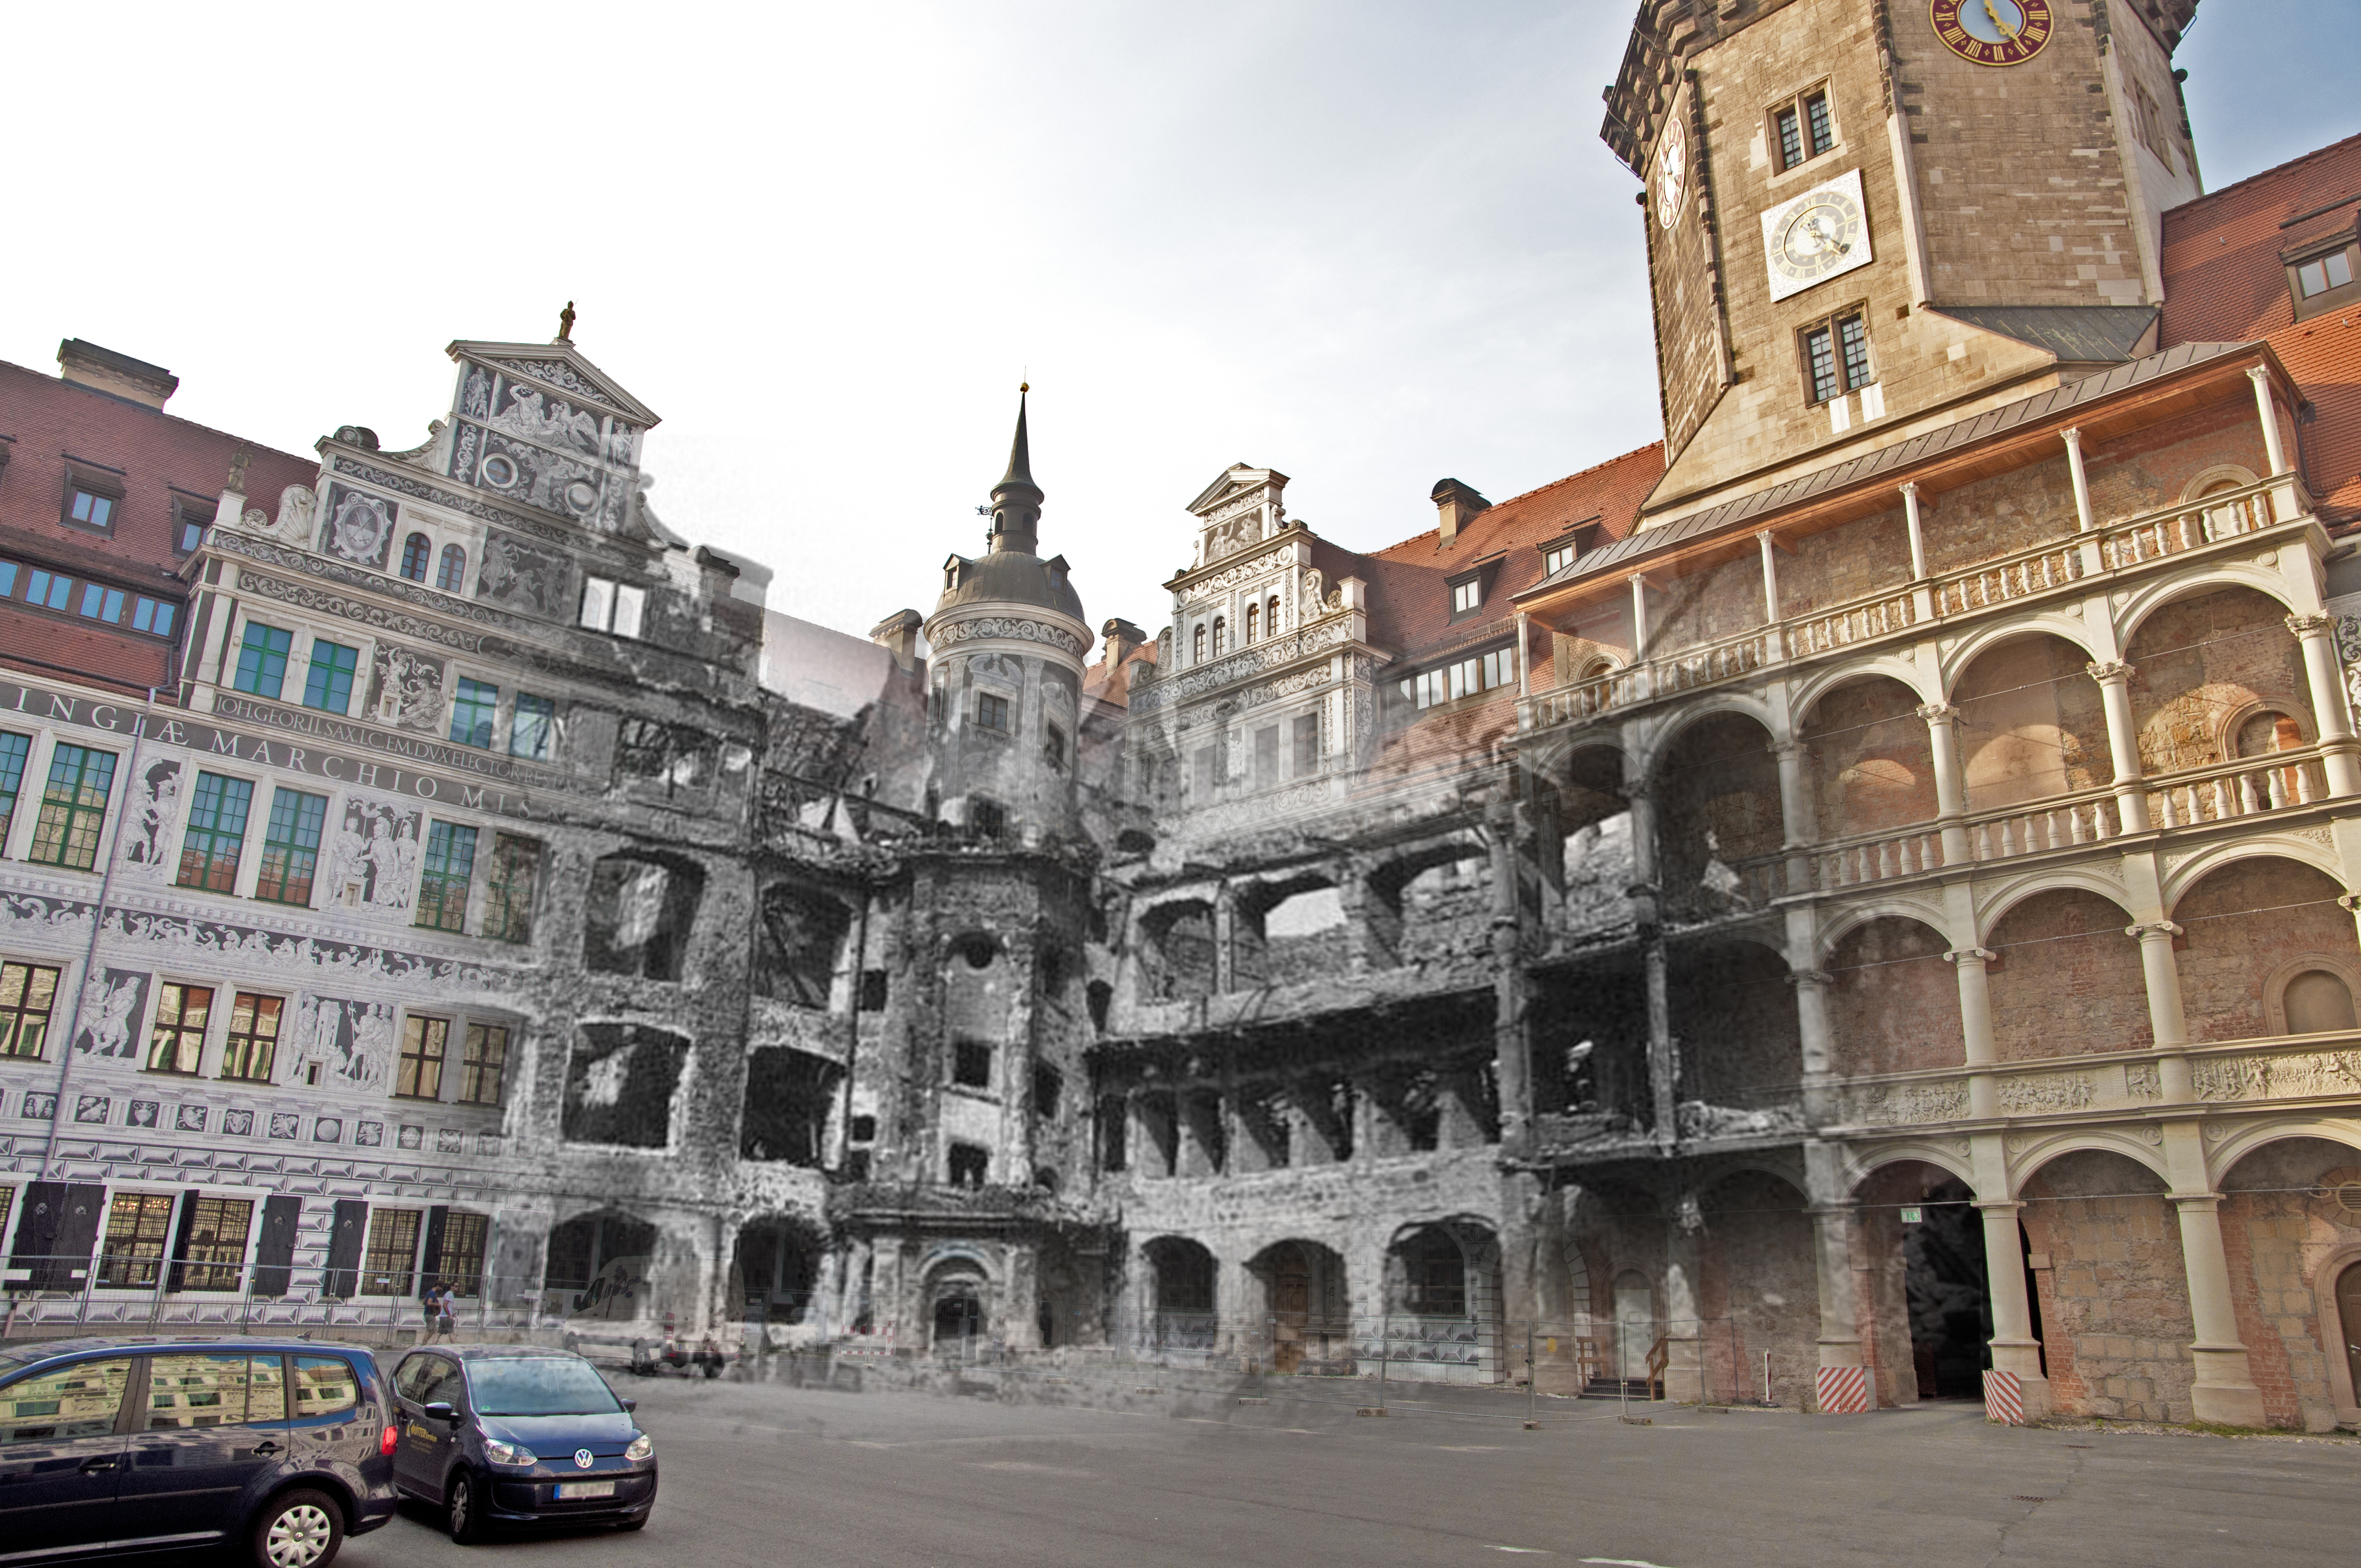
\includegraphics[width=\textwidth]{gfx/1945_2014_Residenzschloss.jpg}
   \caption{Residenzschloss in Dresden, destroyed during World War II,
   \textcopyright\ Sergey Larenkov, printed with permission}
   \label{fig1}
\end{figure}

\begin{figure}
   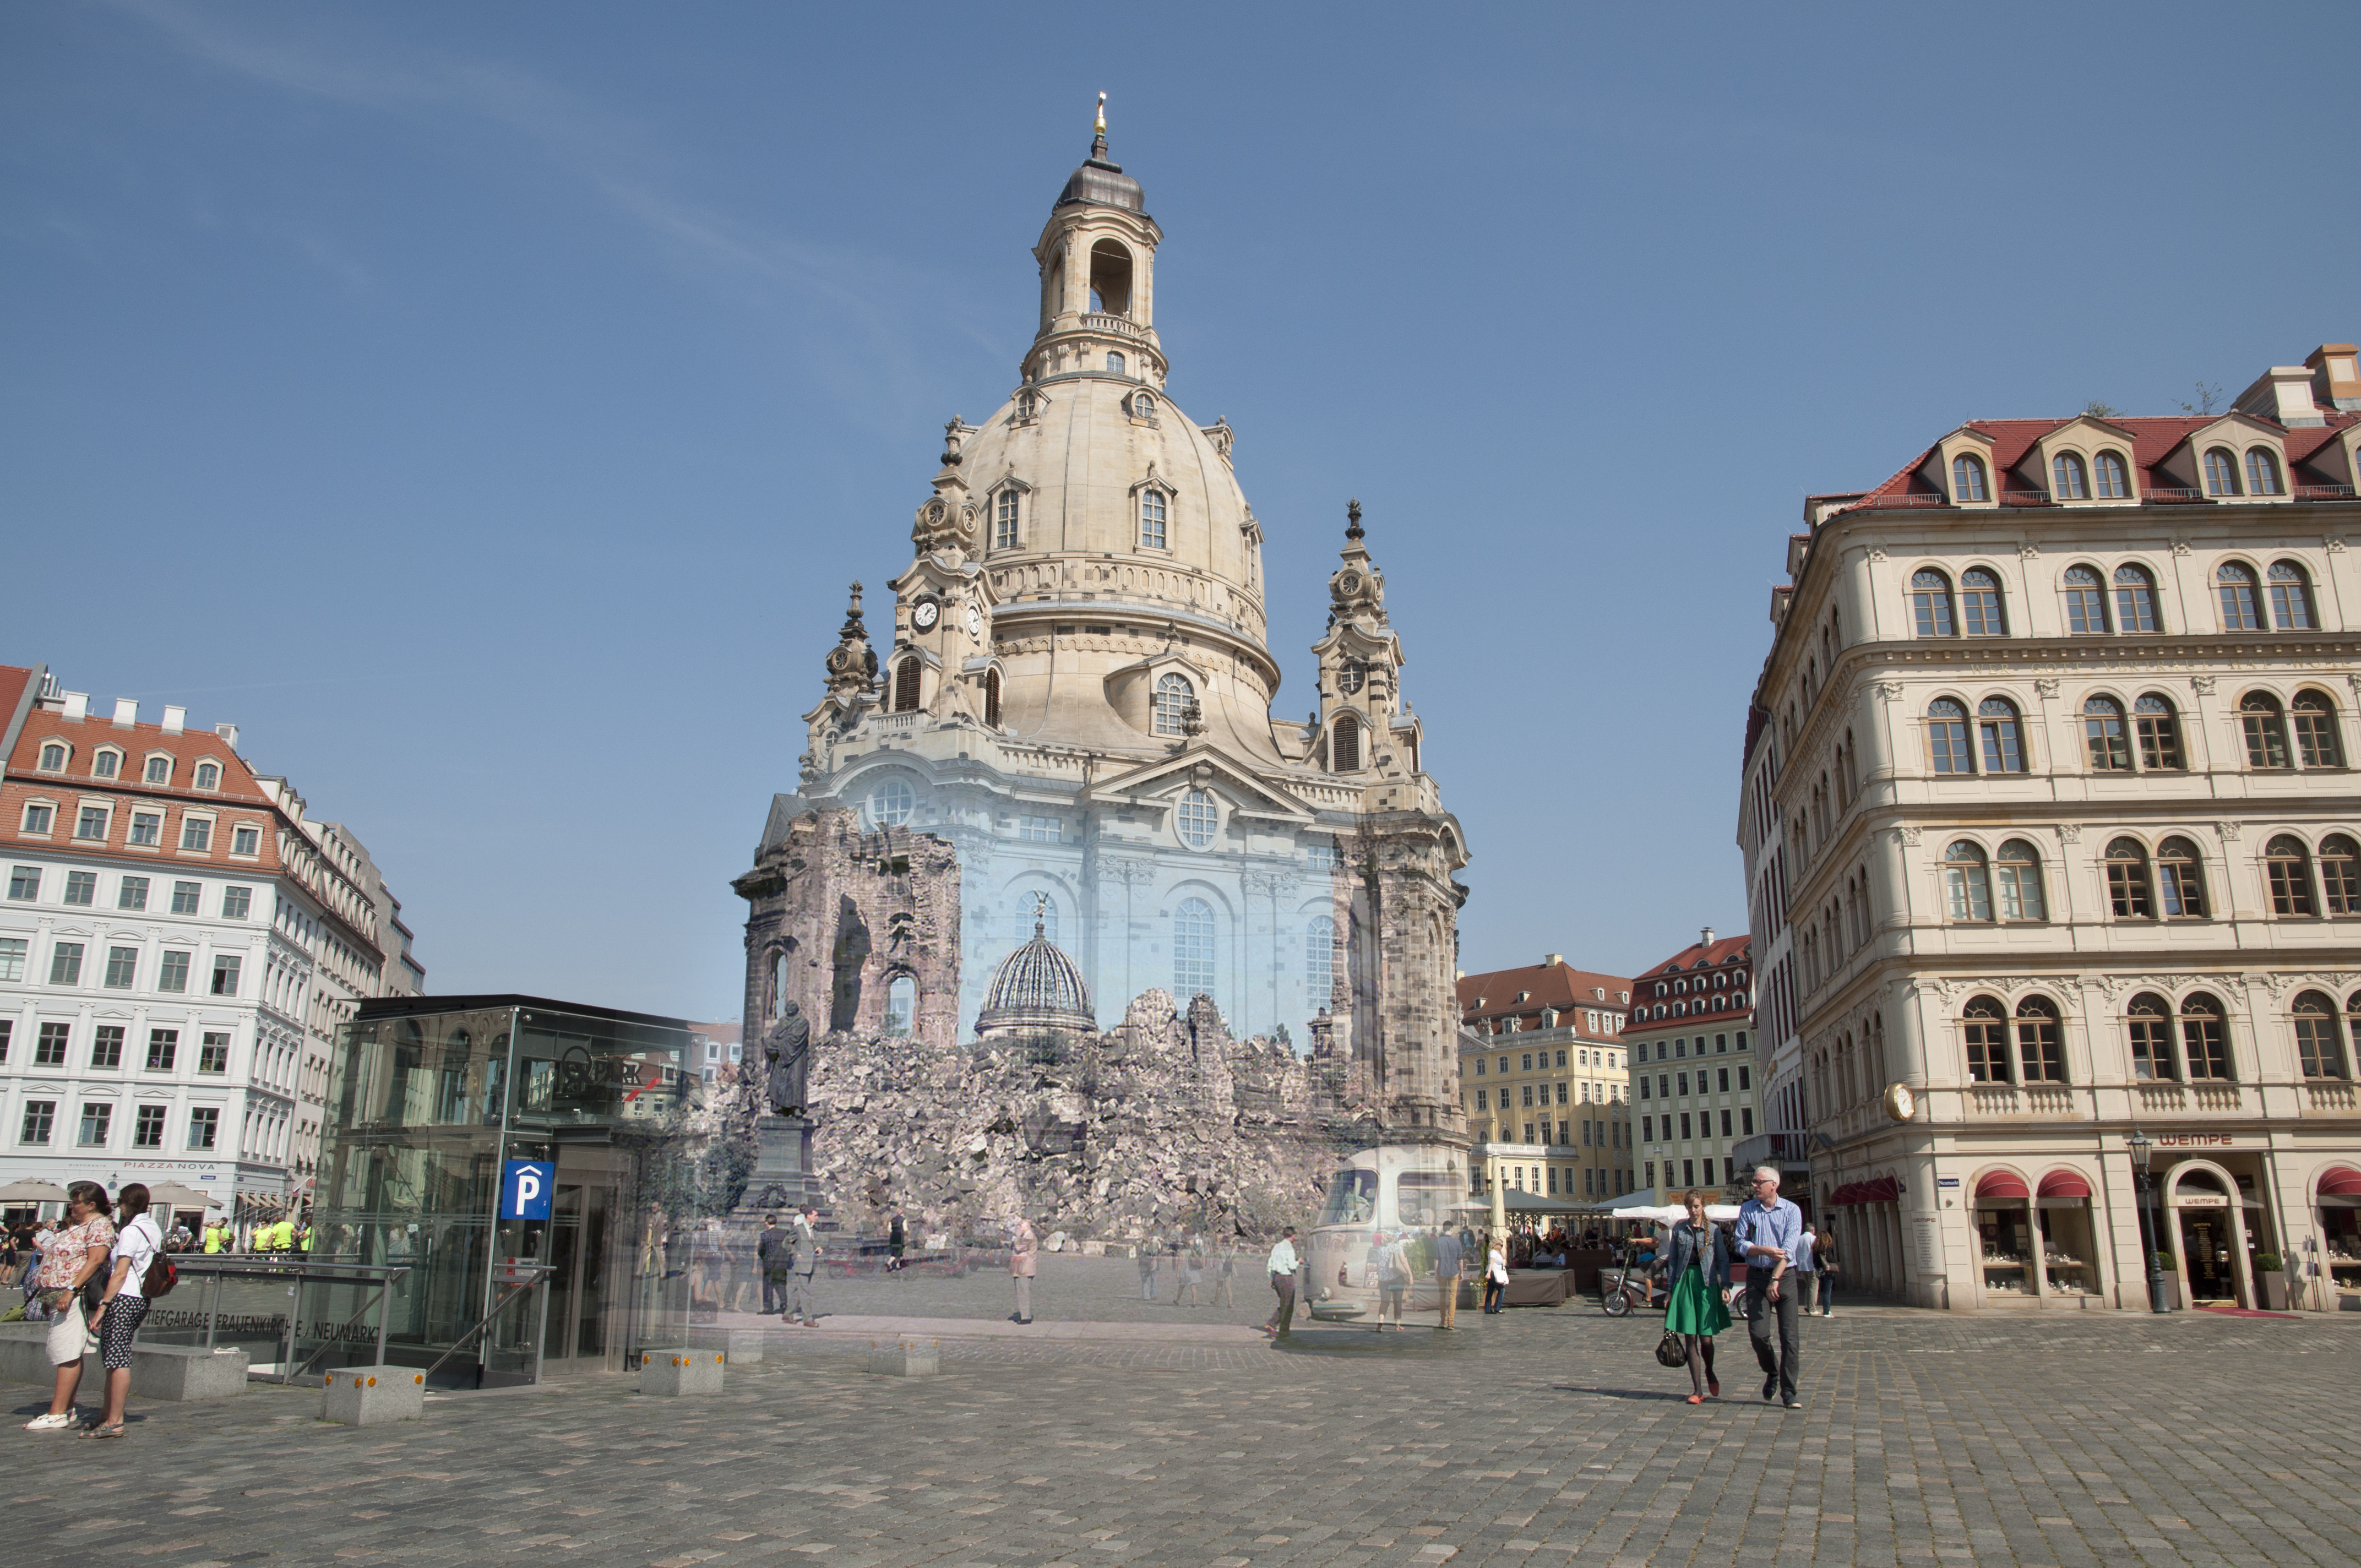
\includegraphics[width=\textwidth]{gfx/1950_2014_Frauenkirche.jpg}
   \caption{Frauenkirche in Dresden, destroyed during World War II,
   \textcopyright\ Sergey Larenkov, printed with permission}
   \label{fig2}
\end{figure}

When done manually, the photographer must attempt to find the original viewpoint 
usually by visual inspection of the original image and trying to match the
current camera parameters --- camera position, camera rotation, focal length,
possibly principal point --- to the original.
The procedure is often carried out by placing the camera on a tripod and
comparing a printout of the original image with what can be seen through the
viewfinder or the camera screen. The number of parameters to match as well as
the difficulty to estimate them purely from comparing two-dimensional images makes the process
error-prone and tedious. Visual acuity and experience of the photographer thus
place limits on the accuracy with which the camera pose of the reference image
can be reconstructed. 

The advancement of mobile phones anc tablet computers with integrated cameras
and larger screens presents the opportunity to develop applications which can
assist in this endeavour, moving away from the traditional trial-and-error
approach.  On current digital cameras\footnote{At the time of writing, no
   commercial manufacturer produces a camera with user-modifiable firm- or
software. A project at Stanford \citep{Levoy2010} was discontinued
\cite{FrankenCam}} this is impossible due to their closed infrastructure not
permitting running user programs. 

\section{Previous Approaches}

Several applications have been developed to assist a photographer in taking
rephotographs. For smartphone operating systems,
\emph{rePhoto}\footnote{\url{http://projectrephoto.com/}} and
\emph{Timera}\footnote{\url{http://www.timera.com/Explore}} exist, both
available for Android and iOS devices. These applications support the user by placing a transparent
version of the original image over the current camera image, allowing for easier
alignment. The captured rephotograph is then presented together with the
original image in a blend (c.f. \autoref{fig3}).

What is characteristical about both applications is that the user must still
determine on their own how to actually move the camera. An overlay simplifies
the procedure, eliminating some of the inaccuracy introduced into the manual approach by the
necessity to move the eyes from printout to camera, but it is still the user's
responsibility to determine the necessary motion between the current camera
position and the goal position (that of the original image). A more
sophisticated approach was presented in \citep{bae2010} by Bae et al.


